
% Default to the notebook output style

    


% Inherit from the specified cell style.




    
\documentclass[11pt]{article}

    
    
    \usepackage[T1]{fontenc}
    % Nicer default font than Computer Modern for most use cases
    \usepackage{palatino}

    % Basic figure setup, for now with no caption control since it's done
    % automatically by Pandoc (which extracts ![](path) syntax from Markdown).
    \usepackage{graphicx}
    % We will generate all images so they have a width \maxwidth. This means
    % that they will get their normal width if they fit onto the page, but
    % are scaled down if they would overflow the margins.
    \makeatletter
    \def\maxwidth{\ifdim\Gin@nat@width>\linewidth\linewidth
    \else\Gin@nat@width\fi}
    \makeatother
    \let\Oldincludegraphics\includegraphics
    % Set max figure width to be 80% of text width, for now hardcoded.
    \renewcommand{\includegraphics}[1]{\Oldincludegraphics[width=.8\maxwidth]{#1}}
    % Ensure that by default, figures have no caption (until we provide a
    % proper Figure object with a Caption API and a way to capture that
    % in the conversion process - todo).
    \usepackage{caption}
    \DeclareCaptionLabelFormat{nolabel}{}
    \captionsetup{labelformat=nolabel}

    \usepackage{adjustbox} % Used to constrain images to a maximum size 
    \usepackage{xcolor} % Allow colors to be defined
    \usepackage{enumerate} % Needed for markdown enumerations to work
    \usepackage{geometry} % Used to adjust the document margins
    \usepackage{amsmath} % Equations
    \usepackage{amssymb} % Equations
    \usepackage{textcomp} % defines textquotesingle
    % Hack from http://tex.stackexchange.com/a/47451/13684:
    \AtBeginDocument{%
        \def\PYZsq{\textquotesingle}% Upright quotes in Pygmentized code
    }
    \usepackage{upquote} % Upright quotes for verbatim code
    \usepackage{eurosym} % defines \euro
    \usepackage[mathletters]{ucs} % Extended unicode (utf-8) support
    \usepackage[utf8x]{inputenc} % Allow utf-8 characters in the tex document
    \usepackage{fancyvrb} % verbatim replacement that allows latex
    \usepackage{grffile} % extends the file name processing of package graphics 
                         % to support a larger range 
    % The hyperref package gives us a pdf with properly built
    % internal navigation ('pdf bookmarks' for the table of contents,
    % internal cross-reference links, web links for URLs, etc.)
    \usepackage{hyperref}
    \usepackage{longtable} % longtable support required by pandoc >1.10
    \usepackage{booktabs}  % table support for pandoc > 1.12.2
    \usepackage[normalem]{ulem} % ulem is needed to support strikethroughs (\sout)
                                % normalem makes italics be italics, not underlines
    

    
    
    % Colors for the hyperref package
    \definecolor{urlcolor}{rgb}{0,.145,.698}
    \definecolor{linkcolor}{rgb}{.71,0.21,0.01}
    \definecolor{citecolor}{rgb}{.12,.54,.11}

    % ANSI colors
    \definecolor{ansi-black}{HTML}{3E424D}
    \definecolor{ansi-black-intense}{HTML}{282C36}
    \definecolor{ansi-red}{HTML}{E75C58}
    \definecolor{ansi-red-intense}{HTML}{B22B31}
    \definecolor{ansi-green}{HTML}{00A250}
    \definecolor{ansi-green-intense}{HTML}{007427}
    \definecolor{ansi-yellow}{HTML}{DDB62B}
    \definecolor{ansi-yellow-intense}{HTML}{B27D12}
    \definecolor{ansi-blue}{HTML}{208FFB}
    \definecolor{ansi-blue-intense}{HTML}{0065CA}
    \definecolor{ansi-magenta}{HTML}{D160C4}
    \definecolor{ansi-magenta-intense}{HTML}{A03196}
    \definecolor{ansi-cyan}{HTML}{60C6C8}
    \definecolor{ansi-cyan-intense}{HTML}{258F8F}
    \definecolor{ansi-white}{HTML}{C5C1B4}
    \definecolor{ansi-white-intense}{HTML}{A1A6B2}

    % commands and environments needed by pandoc snippets
    % extracted from the output of `pandoc -s`
    \providecommand{\tightlist}{%
      \setlength{\itemsep}{0pt}\setlength{\parskip}{0pt}}
    \DefineVerbatimEnvironment{Highlighting}{Verbatim}{commandchars=\\\{\}}
    % Add ',fontsize=\small' for more characters per line
    \newenvironment{Shaded}{}{}
    \newcommand{\KeywordTok}[1]{\textcolor[rgb]{0.00,0.44,0.13}{\textbf{{#1}}}}
    \newcommand{\DataTypeTok}[1]{\textcolor[rgb]{0.56,0.13,0.00}{{#1}}}
    \newcommand{\DecValTok}[1]{\textcolor[rgb]{0.25,0.63,0.44}{{#1}}}
    \newcommand{\BaseNTok}[1]{\textcolor[rgb]{0.25,0.63,0.44}{{#1}}}
    \newcommand{\FloatTok}[1]{\textcolor[rgb]{0.25,0.63,0.44}{{#1}}}
    \newcommand{\CharTok}[1]{\textcolor[rgb]{0.25,0.44,0.63}{{#1}}}
    \newcommand{\StringTok}[1]{\textcolor[rgb]{0.25,0.44,0.63}{{#1}}}
    \newcommand{\CommentTok}[1]{\textcolor[rgb]{0.38,0.63,0.69}{\textit{{#1}}}}
    \newcommand{\OtherTok}[1]{\textcolor[rgb]{0.00,0.44,0.13}{{#1}}}
    \newcommand{\AlertTok}[1]{\textcolor[rgb]{1.00,0.00,0.00}{\textbf{{#1}}}}
    \newcommand{\FunctionTok}[1]{\textcolor[rgb]{0.02,0.16,0.49}{{#1}}}
    \newcommand{\RegionMarkerTok}[1]{{#1}}
    \newcommand{\ErrorTok}[1]{\textcolor[rgb]{1.00,0.00,0.00}{\textbf{{#1}}}}
    \newcommand{\NormalTok}[1]{{#1}}
    
    % Additional commands for more recent versions of Pandoc
    \newcommand{\ConstantTok}[1]{\textcolor[rgb]{0.53,0.00,0.00}{{#1}}}
    \newcommand{\SpecialCharTok}[1]{\textcolor[rgb]{0.25,0.44,0.63}{{#1}}}
    \newcommand{\VerbatimStringTok}[1]{\textcolor[rgb]{0.25,0.44,0.63}{{#1}}}
    \newcommand{\SpecialStringTok}[1]{\textcolor[rgb]{0.73,0.40,0.53}{{#1}}}
    \newcommand{\ImportTok}[1]{{#1}}
    \newcommand{\DocumentationTok}[1]{\textcolor[rgb]{0.73,0.13,0.13}{\textit{{#1}}}}
    \newcommand{\AnnotationTok}[1]{\textcolor[rgb]{0.38,0.63,0.69}{\textbf{\textit{{#1}}}}}
    \newcommand{\CommentVarTok}[1]{\textcolor[rgb]{0.38,0.63,0.69}{\textbf{\textit{{#1}}}}}
    \newcommand{\VariableTok}[1]{\textcolor[rgb]{0.10,0.09,0.49}{{#1}}}
    \newcommand{\ControlFlowTok}[1]{\textcolor[rgb]{0.00,0.44,0.13}{\textbf{{#1}}}}
    \newcommand{\OperatorTok}[1]{\textcolor[rgb]{0.40,0.40,0.40}{{#1}}}
    \newcommand{\BuiltInTok}[1]{{#1}}
    \newcommand{\ExtensionTok}[1]{{#1}}
    \newcommand{\PreprocessorTok}[1]{\textcolor[rgb]{0.74,0.48,0.00}{{#1}}}
    \newcommand{\AttributeTok}[1]{\textcolor[rgb]{0.49,0.56,0.16}{{#1}}}
    \newcommand{\InformationTok}[1]{\textcolor[rgb]{0.38,0.63,0.69}{\textbf{\textit{{#1}}}}}
    \newcommand{\WarningTok}[1]{\textcolor[rgb]{0.38,0.63,0.69}{\textbf{\textit{{#1}}}}}
    
    
    % Define a nice break command that doesn't care if a line doesn't already
    % exist.
    \def\br{\hspace*{\fill} \\* }
    % Math Jax compatability definitions
    \def\gt{>}
    \def\lt{<}
    % Document parameters
    \title{Titanic Dataset Analysis}
    
    
    

    % Pygments definitions
    
\makeatletter
\def\PY@reset{\let\PY@it=\relax \let\PY@bf=\relax%
    \let\PY@ul=\relax \let\PY@tc=\relax%
    \let\PY@bc=\relax \let\PY@ff=\relax}
\def\PY@tok#1{\csname PY@tok@#1\endcsname}
\def\PY@toks#1+{\ifx\relax#1\empty\else%
    \PY@tok{#1}\expandafter\PY@toks\fi}
\def\PY@do#1{\PY@bc{\PY@tc{\PY@ul{%
    \PY@it{\PY@bf{\PY@ff{#1}}}}}}}
\def\PY#1#2{\PY@reset\PY@toks#1+\relax+\PY@do{#2}}

\expandafter\def\csname PY@tok@gd\endcsname{\def\PY@tc##1{\textcolor[rgb]{0.63,0.00,0.00}{##1}}}
\expandafter\def\csname PY@tok@gu\endcsname{\let\PY@bf=\textbf\def\PY@tc##1{\textcolor[rgb]{0.50,0.00,0.50}{##1}}}
\expandafter\def\csname PY@tok@gt\endcsname{\def\PY@tc##1{\textcolor[rgb]{0.00,0.27,0.87}{##1}}}
\expandafter\def\csname PY@tok@gs\endcsname{\let\PY@bf=\textbf}
\expandafter\def\csname PY@tok@gr\endcsname{\def\PY@tc##1{\textcolor[rgb]{1.00,0.00,0.00}{##1}}}
\expandafter\def\csname PY@tok@cm\endcsname{\let\PY@it=\textit\def\PY@tc##1{\textcolor[rgb]{0.25,0.50,0.50}{##1}}}
\expandafter\def\csname PY@tok@vg\endcsname{\def\PY@tc##1{\textcolor[rgb]{0.10,0.09,0.49}{##1}}}
\expandafter\def\csname PY@tok@vi\endcsname{\def\PY@tc##1{\textcolor[rgb]{0.10,0.09,0.49}{##1}}}
\expandafter\def\csname PY@tok@mh\endcsname{\def\PY@tc##1{\textcolor[rgb]{0.40,0.40,0.40}{##1}}}
\expandafter\def\csname PY@tok@cs\endcsname{\let\PY@it=\textit\def\PY@tc##1{\textcolor[rgb]{0.25,0.50,0.50}{##1}}}
\expandafter\def\csname PY@tok@ge\endcsname{\let\PY@it=\textit}
\expandafter\def\csname PY@tok@vc\endcsname{\def\PY@tc##1{\textcolor[rgb]{0.10,0.09,0.49}{##1}}}
\expandafter\def\csname PY@tok@il\endcsname{\def\PY@tc##1{\textcolor[rgb]{0.40,0.40,0.40}{##1}}}
\expandafter\def\csname PY@tok@go\endcsname{\def\PY@tc##1{\textcolor[rgb]{0.53,0.53,0.53}{##1}}}
\expandafter\def\csname PY@tok@cp\endcsname{\def\PY@tc##1{\textcolor[rgb]{0.74,0.48,0.00}{##1}}}
\expandafter\def\csname PY@tok@gi\endcsname{\def\PY@tc##1{\textcolor[rgb]{0.00,0.63,0.00}{##1}}}
\expandafter\def\csname PY@tok@gh\endcsname{\let\PY@bf=\textbf\def\PY@tc##1{\textcolor[rgb]{0.00,0.00,0.50}{##1}}}
\expandafter\def\csname PY@tok@ni\endcsname{\let\PY@bf=\textbf\def\PY@tc##1{\textcolor[rgb]{0.60,0.60,0.60}{##1}}}
\expandafter\def\csname PY@tok@nl\endcsname{\def\PY@tc##1{\textcolor[rgb]{0.63,0.63,0.00}{##1}}}
\expandafter\def\csname PY@tok@nn\endcsname{\let\PY@bf=\textbf\def\PY@tc##1{\textcolor[rgb]{0.00,0.00,1.00}{##1}}}
\expandafter\def\csname PY@tok@no\endcsname{\def\PY@tc##1{\textcolor[rgb]{0.53,0.00,0.00}{##1}}}
\expandafter\def\csname PY@tok@na\endcsname{\def\PY@tc##1{\textcolor[rgb]{0.49,0.56,0.16}{##1}}}
\expandafter\def\csname PY@tok@nb\endcsname{\def\PY@tc##1{\textcolor[rgb]{0.00,0.50,0.00}{##1}}}
\expandafter\def\csname PY@tok@nc\endcsname{\let\PY@bf=\textbf\def\PY@tc##1{\textcolor[rgb]{0.00,0.00,1.00}{##1}}}
\expandafter\def\csname PY@tok@nd\endcsname{\def\PY@tc##1{\textcolor[rgb]{0.67,0.13,1.00}{##1}}}
\expandafter\def\csname PY@tok@ne\endcsname{\let\PY@bf=\textbf\def\PY@tc##1{\textcolor[rgb]{0.82,0.25,0.23}{##1}}}
\expandafter\def\csname PY@tok@nf\endcsname{\def\PY@tc##1{\textcolor[rgb]{0.00,0.00,1.00}{##1}}}
\expandafter\def\csname PY@tok@si\endcsname{\let\PY@bf=\textbf\def\PY@tc##1{\textcolor[rgb]{0.73,0.40,0.53}{##1}}}
\expandafter\def\csname PY@tok@s2\endcsname{\def\PY@tc##1{\textcolor[rgb]{0.73,0.13,0.13}{##1}}}
\expandafter\def\csname PY@tok@nt\endcsname{\let\PY@bf=\textbf\def\PY@tc##1{\textcolor[rgb]{0.00,0.50,0.00}{##1}}}
\expandafter\def\csname PY@tok@nv\endcsname{\def\PY@tc##1{\textcolor[rgb]{0.10,0.09,0.49}{##1}}}
\expandafter\def\csname PY@tok@s1\endcsname{\def\PY@tc##1{\textcolor[rgb]{0.73,0.13,0.13}{##1}}}
\expandafter\def\csname PY@tok@ch\endcsname{\let\PY@it=\textit\def\PY@tc##1{\textcolor[rgb]{0.25,0.50,0.50}{##1}}}
\expandafter\def\csname PY@tok@m\endcsname{\def\PY@tc##1{\textcolor[rgb]{0.40,0.40,0.40}{##1}}}
\expandafter\def\csname PY@tok@gp\endcsname{\let\PY@bf=\textbf\def\PY@tc##1{\textcolor[rgb]{0.00,0.00,0.50}{##1}}}
\expandafter\def\csname PY@tok@sh\endcsname{\def\PY@tc##1{\textcolor[rgb]{0.73,0.13,0.13}{##1}}}
\expandafter\def\csname PY@tok@ow\endcsname{\let\PY@bf=\textbf\def\PY@tc##1{\textcolor[rgb]{0.67,0.13,1.00}{##1}}}
\expandafter\def\csname PY@tok@sx\endcsname{\def\PY@tc##1{\textcolor[rgb]{0.00,0.50,0.00}{##1}}}
\expandafter\def\csname PY@tok@bp\endcsname{\def\PY@tc##1{\textcolor[rgb]{0.00,0.50,0.00}{##1}}}
\expandafter\def\csname PY@tok@c1\endcsname{\let\PY@it=\textit\def\PY@tc##1{\textcolor[rgb]{0.25,0.50,0.50}{##1}}}
\expandafter\def\csname PY@tok@o\endcsname{\def\PY@tc##1{\textcolor[rgb]{0.40,0.40,0.40}{##1}}}
\expandafter\def\csname PY@tok@kc\endcsname{\let\PY@bf=\textbf\def\PY@tc##1{\textcolor[rgb]{0.00,0.50,0.00}{##1}}}
\expandafter\def\csname PY@tok@c\endcsname{\let\PY@it=\textit\def\PY@tc##1{\textcolor[rgb]{0.25,0.50,0.50}{##1}}}
\expandafter\def\csname PY@tok@mf\endcsname{\def\PY@tc##1{\textcolor[rgb]{0.40,0.40,0.40}{##1}}}
\expandafter\def\csname PY@tok@err\endcsname{\def\PY@bc##1{\setlength{\fboxsep}{0pt}\fcolorbox[rgb]{1.00,0.00,0.00}{1,1,1}{\strut ##1}}}
\expandafter\def\csname PY@tok@mb\endcsname{\def\PY@tc##1{\textcolor[rgb]{0.40,0.40,0.40}{##1}}}
\expandafter\def\csname PY@tok@ss\endcsname{\def\PY@tc##1{\textcolor[rgb]{0.10,0.09,0.49}{##1}}}
\expandafter\def\csname PY@tok@sr\endcsname{\def\PY@tc##1{\textcolor[rgb]{0.73,0.40,0.53}{##1}}}
\expandafter\def\csname PY@tok@mo\endcsname{\def\PY@tc##1{\textcolor[rgb]{0.40,0.40,0.40}{##1}}}
\expandafter\def\csname PY@tok@kd\endcsname{\let\PY@bf=\textbf\def\PY@tc##1{\textcolor[rgb]{0.00,0.50,0.00}{##1}}}
\expandafter\def\csname PY@tok@mi\endcsname{\def\PY@tc##1{\textcolor[rgb]{0.40,0.40,0.40}{##1}}}
\expandafter\def\csname PY@tok@kn\endcsname{\let\PY@bf=\textbf\def\PY@tc##1{\textcolor[rgb]{0.00,0.50,0.00}{##1}}}
\expandafter\def\csname PY@tok@cpf\endcsname{\let\PY@it=\textit\def\PY@tc##1{\textcolor[rgb]{0.25,0.50,0.50}{##1}}}
\expandafter\def\csname PY@tok@kr\endcsname{\let\PY@bf=\textbf\def\PY@tc##1{\textcolor[rgb]{0.00,0.50,0.00}{##1}}}
\expandafter\def\csname PY@tok@s\endcsname{\def\PY@tc##1{\textcolor[rgb]{0.73,0.13,0.13}{##1}}}
\expandafter\def\csname PY@tok@kp\endcsname{\def\PY@tc##1{\textcolor[rgb]{0.00,0.50,0.00}{##1}}}
\expandafter\def\csname PY@tok@w\endcsname{\def\PY@tc##1{\textcolor[rgb]{0.73,0.73,0.73}{##1}}}
\expandafter\def\csname PY@tok@kt\endcsname{\def\PY@tc##1{\textcolor[rgb]{0.69,0.00,0.25}{##1}}}
\expandafter\def\csname PY@tok@sc\endcsname{\def\PY@tc##1{\textcolor[rgb]{0.73,0.13,0.13}{##1}}}
\expandafter\def\csname PY@tok@sb\endcsname{\def\PY@tc##1{\textcolor[rgb]{0.73,0.13,0.13}{##1}}}
\expandafter\def\csname PY@tok@k\endcsname{\let\PY@bf=\textbf\def\PY@tc##1{\textcolor[rgb]{0.00,0.50,0.00}{##1}}}
\expandafter\def\csname PY@tok@se\endcsname{\let\PY@bf=\textbf\def\PY@tc##1{\textcolor[rgb]{0.73,0.40,0.13}{##1}}}
\expandafter\def\csname PY@tok@sd\endcsname{\let\PY@it=\textit\def\PY@tc##1{\textcolor[rgb]{0.73,0.13,0.13}{##1}}}

\def\PYZbs{\char`\\}
\def\PYZus{\char`\_}
\def\PYZob{\char`\{}
\def\PYZcb{\char`\}}
\def\PYZca{\char`\^}
\def\PYZam{\char`\&}
\def\PYZlt{\char`\<}
\def\PYZgt{\char`\>}
\def\PYZsh{\char`\#}
\def\PYZpc{\char`\%}
\def\PYZdl{\char`\$}
\def\PYZhy{\char`\-}
\def\PYZsq{\char`\'}
\def\PYZdq{\char`\"}
\def\PYZti{\char`\~}
% for compatibility with earlier versions
\def\PYZat{@}
\def\PYZlb{[}
\def\PYZrb{]}
\makeatother


    % Exact colors from NB
    \definecolor{incolor}{rgb}{0.0, 0.0, 0.5}
    \definecolor{outcolor}{rgb}{0.545, 0.0, 0.0}



    
    % Prevent overflowing lines due to hard-to-break entities
    \sloppy 
    % Setup hyperref package
    \hypersetup{
      breaklinks=true,  % so long urls are correctly broken across lines
      colorlinks=true,
      urlcolor=urlcolor,
      linkcolor=linkcolor,
      citecolor=citecolor,
      }
    % Slightly bigger margins than the latex defaults
    
    \geometry{verbose,tmargin=1in,bmargin=1in,lmargin=1in,rmargin=1in}
    
    

    \begin{document}
    
    
    \maketitle
    
    

    
    \section{Titanic Dataset Analysis}\label{titanic-dataset-analysis}

Creation Date:21/07/2017

\textbf{Author}: Mamadou Diallo

Source code for analysis (separate file): `\textbf{\emph{Titanic Dataset
Notebook Coding.ipynb}}'

    \subsection{Dataset selected}\label{dataset-selected}

In the frame of Udacity Data Analyst Nanodegree this project is
conducted using the Titanic Dataset found
\href{https://d17h27t6h515a5.cloudfront.net/topher/2016/September/57e9a84c_titanic-data/titanic-data.csv}{here}

The kaggle site - cf. {[}kaggleTitanic{]} in documentation section -
contains the original source of the data and its description.

    \subsection{Questions}\label{questions}

\textbf{Q1. What are the most important factors to survival (e.g.~Sex,
Class, \ldots{})}

\textbf{Q2. Did they apply the protocol ``Women and Children first''?}

\textbf{Q3. Is there any linear correlation among factors?}

\textbf{Q4. How to deal with missing values?}

    \subsection{Approach to investigate the
questions}\label{approach-to-investigate-the-questions}

\begin{itemize}
\item
  Q1: Use of grouping techniques by categories (e.g.~Sex, Embarked,
  etc.). We will use programming based on document {[}Hdbk{]}. We'll use
  plots with the help of document {[}Plot{]}.
\item
  Q2: The computation of the survival numbers by category (e.g.~Sex,
  Embarked) and investigation (such as Document {[}Wikipedia{]}) if the
  protocol was enforced.
\item
  Q3: The use of the Pearson's correlation matrix would be usefull. And
  an example is provided in document {[}HM{]}
\item
  Q4: Measure the \% of missing values per feature (i.e.~variable). Use
  of articles on the subject such as document {[}MV{]}.
\end{itemize}

    \subsection{Data Description}\label{data-description}

The following Data Dictionary is given from Document {[}kaggleTitanic{]}

\begin{longtable}[]{@{}lll@{}}
\toprule
\begin{minipage}[b]{0.18\columnwidth}\raggedright\strut
Variable\strut
\end{minipage} & \begin{minipage}[b]{0.18\columnwidth}\raggedright\strut
Definition\strut
\end{minipage} & \begin{minipage}[b]{0.18\columnwidth}\raggedright\strut
Key\strut
\end{minipage}\tabularnewline
\midrule
\endhead
\begin{minipage}[t]{0.18\columnwidth}\raggedright\strut
survival\strut
\end{minipage} & \begin{minipage}[t]{0.18\columnwidth}\raggedright\strut
Survival\strut
\end{minipage} & \begin{minipage}[t]{0.18\columnwidth}\raggedright\strut
0 = No, 1 = Yes\strut
\end{minipage}\tabularnewline
\begin{minipage}[t]{0.18\columnwidth}\raggedright\strut
pclass\strut
\end{minipage} & \begin{minipage}[t]{0.18\columnwidth}\raggedright\strut
Ticket class\strut
\end{minipage} & \begin{minipage}[t]{0.18\columnwidth}\raggedright\strut
1 = 1st, 2 = 2nd, 3 = 3rd\strut
\end{minipage}\tabularnewline
\begin{minipage}[t]{0.18\columnwidth}\raggedright\strut
Sex\strut
\end{minipage} & \begin{minipage}[t]{0.18\columnwidth}\raggedright\strut
Sex\strut
\end{minipage} & \begin{minipage}[t]{0.18\columnwidth}\raggedright\strut
male/female\strut
\end{minipage}\tabularnewline
\begin{minipage}[t]{0.18\columnwidth}\raggedright\strut
Age\strut
\end{minipage} & \begin{minipage}[t]{0.18\columnwidth}\raggedright\strut
Age\strut
\end{minipage} & \begin{minipage}[t]{0.18\columnwidth}\raggedright\strut
in years\strut
\end{minipage}\tabularnewline
\begin{minipage}[t]{0.18\columnwidth}\raggedright\strut
sibsp\strut
\end{minipage} & \begin{minipage}[t]{0.18\columnwidth}\raggedright\strut
\# of siblings / spouses aboard the Titanic\strut
\end{minipage} & \begin{minipage}[t]{0.18\columnwidth}\raggedright\strut
\strut
\end{minipage}\tabularnewline
\begin{minipage}[t]{0.18\columnwidth}\raggedright\strut
parch\strut
\end{minipage} & \begin{minipage}[t]{0.18\columnwidth}\raggedright\strut
\# of parents / children aboard the Titanic\strut
\end{minipage} & \begin{minipage}[t]{0.18\columnwidth}\raggedright\strut
\strut
\end{minipage}\tabularnewline
\begin{minipage}[t]{0.18\columnwidth}\raggedright\strut
ticket\strut
\end{minipage} & \begin{minipage}[t]{0.18\columnwidth}\raggedright\strut
Ticket number\strut
\end{minipage} & \begin{minipage}[t]{0.18\columnwidth}\raggedright\strut
\strut
\end{minipage}\tabularnewline
\begin{minipage}[t]{0.18\columnwidth}\raggedright\strut
fare\strut
\end{minipage} & \begin{minipage}[t]{0.18\columnwidth}\raggedright\strut
Passenger fare\strut
\end{minipage} & \begin{minipage}[t]{0.18\columnwidth}\raggedright\strut
\strut
\end{minipage}\tabularnewline
\begin{minipage}[t]{0.18\columnwidth}\raggedright\strut
cabin\strut
\end{minipage} & \begin{minipage}[t]{0.18\columnwidth}\raggedright\strut
Cabin number\strut
\end{minipage} & \begin{minipage}[t]{0.18\columnwidth}\raggedright\strut
\strut
\end{minipage}\tabularnewline
\begin{minipage}[t]{0.18\columnwidth}\raggedright\strut
embarked\strut
\end{minipage} & \begin{minipage}[t]{0.18\columnwidth}\raggedright\strut
Port of Embarkation\strut
\end{minipage} & \begin{minipage}[t]{0.18\columnwidth}\raggedright\strut
C = Cherbourg, Q = Queenstown, S = Southampton\strut
\end{minipage}\tabularnewline
\bottomrule
\end{longtable}

pclass is A proxy for socio-economic status (SES). 1st = Upper, 2nd =
Middle, 3rd = Lower

Age is fractional if less than 1. If the age is estimated, is it in the
form of xx.5

sibsp: The dataset defines family relations in this way\ldots{} Sibling
= brother, sister, stepbrother, stepsister Spouse = husband, wife
(mistresses and fiancés were ignored)

parch: The dataset defines family relations in this way\ldots{} Parent =
mother, father Child = daughter, son, stepdaughter, stepson Some
children travelled only with a nanny, therefore parch=0 for them.

    \subsection{Data Wrangling}\label{data-wrangling}

To convert and Split nominal features, we use methodology proposed in
document {[}Edx{]}. Pandas .get\_dummies() method allows us to
completely replace a single, nominal feature with multiple boolean
indicator features.

In addition, when analysing the correlation between features it is
preferrable to convert these categorical features into boolean features.

\begin{itemize}
\item
  Sex split into 2 boolean features: `Sex\_female',`Sex\_male'. Done in
  SOURCE CODE \emph{§ Change feature representation for Sex}
\item
  Embarked split into 3 variables boolean features: `Embarked\_C',
  `Embarked\_Q',`Embarked\_S'. Done in SOURCE CODE \emph{§ Change
  feature representation for Embarked}
\item
  We create a new Title feature from Name feature as proposed in
  Document {[}FE{]}. Then we split it into boolean features: Title\_Mr,
  Title\_Master, Title\_Mrs, Title\_Miss. Done in SOURCE CODE \emph{§
  Change feature representation for Title}
\item
  We create the boolean Child feature (passenger with age under 18) to
  answer the question relate Women and Children first protocol. Done in
  SOURCE CODE \emph{§ Build new feature Child}
\end{itemize}

We don't need to consider the following variables for analysing the
relations between features (correlation): - `PassengerId': since it is
replication (shifted by 1) with the line number or the data frame index.
- `Cabin': since there are too little data, we'll skip this feature. -
`Name': Each name is unique - `Ticket': as such, the textual feature is
no use for analysing relation with other features.

\textbf{About missing values:}

We had 3 features - Cabin, Age and Embarked - concerned by missing
values and since the size of the dataset is not large, we did not
consider the deletion of entire observations (rows) containing missing
values. Dealing completely with missing values is part of the questions
(Q4)

    \subsection{Features Study}\label{features-study}

Number of passengers (i.e.~observations) in the data source: 891

On April 15, 1912, the Titanic sank after colliding with an iceberg,
killing 1502 out of 2224 passengers and crew according to document
{[}Wikipedia{]}.

The data provided in document {[}kaggleTitanic{]} shows that it is the
training data. It represents 40\% (i.e.~891/2224) of the overall
population of the Titanic.

In the file, the typical passenger (given by the computation of the mode
of the dataframe): - did not survived - was male - had the title Mr -
was 30 year old. - was in the 3rd class - paid a fare of 8.05 - embarked
at Southampton - had no sibling and no spouse - had no parent

    \subsection{Definitions: Continuous Features vs Categorical
Features}\label{definitions-continuous-features-vs-categorical-features}

Given from Document {[}Edx{]}:

\textbf{Throughout the document, we'll use the word `\emph{feature}'
instead of the word `\emph{variable}'. They can be used
interchangeably.}

\begin{itemize}
\tightlist
\item
  \textbf{Continuous Features}
\end{itemize}

In the case of continuous features, there exist a measurable difference
between possible feature values. Feature values usually are also a
subset of all real numbers:

\begin{itemize}
\tightlist
\item
  \textbf{Categorical Features}
\end{itemize}

With categorical features, there is a specified number of discrete,
possible feature values. These values may or may not have ordering to
them. If they do have a natural ordering, they are called ordinal
categorical features. Otherwise if there is no intrinsic ordering, they
are called nominal categorical features.

\begin{longtable}[]{@{}ll@{}}
\toprule
Example & Type\tabularnewline
\midrule
\endhead
Distance & Continuous\tabularnewline
Time & Continuous\tabularnewline
Cost & Continuous\tabularnewline
Temperature & Continuous\tabularnewline
Car Models & Nominal\tabularnewline
Colors & Nominal\tabularnewline
TV Shows & Nominal\tabularnewline
High-Medium-Low & Ordinal\tabularnewline
1-10 Years Old, 11-20 Years Old, 30-40 Years Old &
Ordinal\tabularnewline
Happy, Neutral, Sad & Ordinal\tabularnewline
\bottomrule
\end{longtable}

    \subsection{Features Study}\label{features-study}

We have 12 features - i.e.~variables - which are either
\textbf{continuous or categorical}.

\textbf{The dependant variable is `Survived' and the rest are
independant variables}.

Categorical features could be split into two sub-types:

ordinal feature or nominal.

    \begin{figure}
\centering
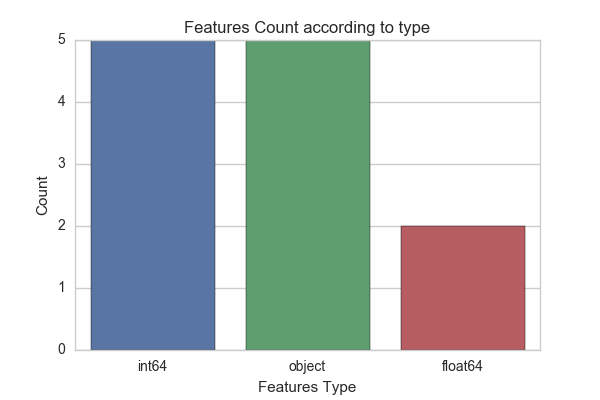
\includegraphics{TypeOfFeatures.png}
\caption{Diagram}
\end{figure}

    \textbf{Two Continuous features are: Age and Fare}

\textbf{\emph{Age}}:

Its type is float64.

\begin{longtable}[]{@{}ll@{}}
\toprule
Variable & Value\tabularnewline
\midrule
\endhead
mode & 30.0\tabularnewline
median & 30.0\tabularnewline
mean & 29.377295\tabularnewline
std & 13.254246\tabularnewline
min & 0.420000\tabularnewline
25\% & 21.000000\tabularnewline
50\% & 30.000000\tabularnewline
75\% & 35.000000\tabularnewline
max & 80.000000\tabularnewline
\bottomrule
\end{longtable}

\begin{figure}
\centering
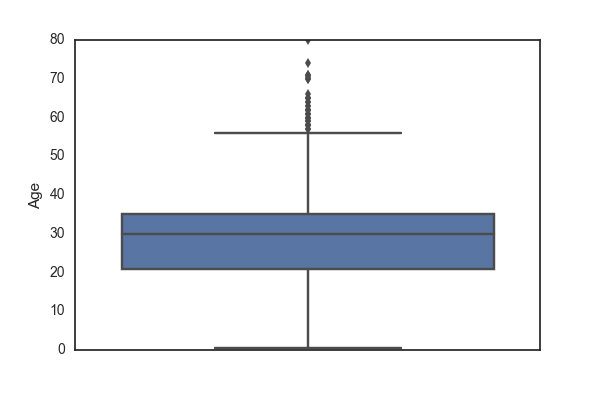
\includegraphics{boxplotAge.png}
\caption{Diagram}
\end{figure}

\textbf{\emph{Fare}}:

Its type is float64.

\begin{longtable}[]{@{}ll@{}}
\toprule
Variable & Value\tabularnewline
\midrule
\endhead
mode & 8.05\tabularnewline
mean & 32.2042079686\tabularnewline
std & 49.6934285972\tabularnewline
min & 0.0\tabularnewline
25\% & 7.910400\tabularnewline
50\% & 14.454200\tabularnewline
75\% & 31.000000\tabularnewline
max & 512.3292\tabularnewline
\bottomrule
\end{longtable}

\begin{figure}
\centering
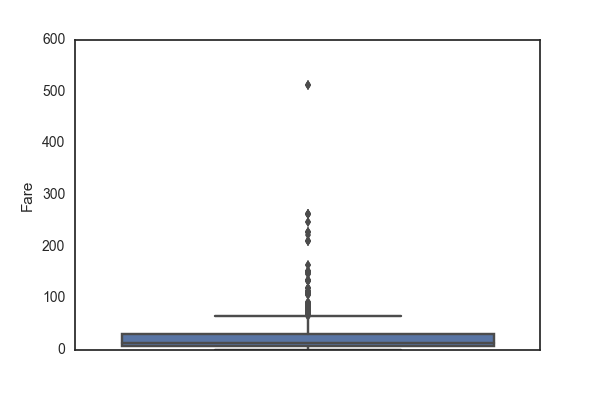
\includegraphics{boxplotFare.png}
\caption{Diagram}
\end{figure}

    \subsubsection{Here below are their
distribution:}\label{here-below-are-their-distribution}

    \begin{figure}
\centering
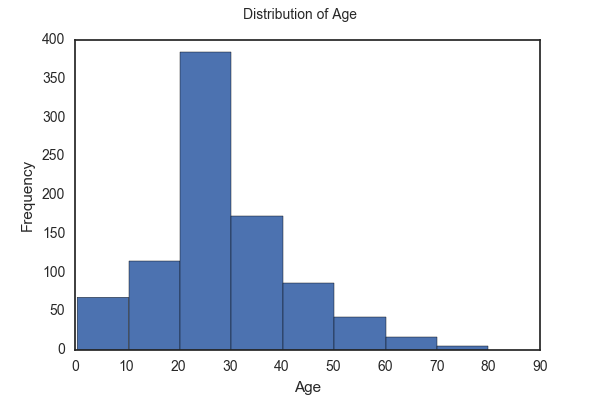
\includegraphics{AgeDistribution.png}
\caption{Diagram}
\end{figure}

    \begin{figure}
\centering
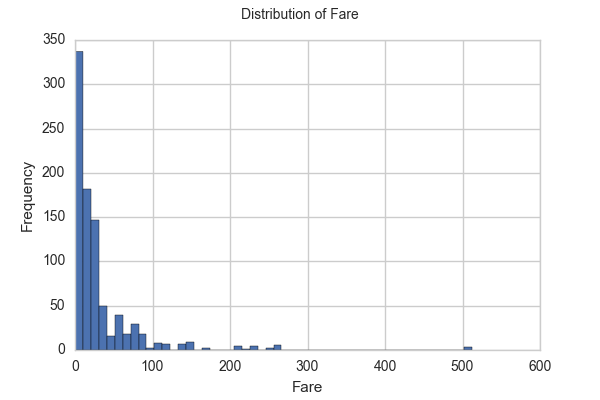
\includegraphics{FareDistribution.png}
\caption{Diagram}
\end{figure}

    The Fare feature distribution is left-skewed (see Fare distribution here
above)

    \subsubsection{\texorpdfstring{Relation Between \emph{Age} and
\emph{Fare}
features}{Relation Between Age and Fare features}}\label{relation-between-age-and-fare-features}

    \begin{figure}
\centering
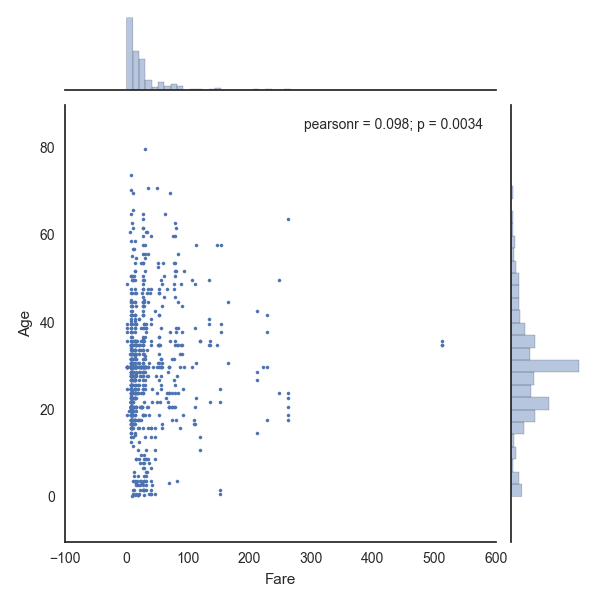
\includegraphics{RelationFarevsAge.png}
\caption{Diagram}
\end{figure}

    There is no relation between the two continuous features (Fare and Age)
as shown here above

    \textbf{Categorical features are:}

`\emph{Pclass}', Ordinal feature (1st class \textgreater{} 2nd Class
\textgreater{} 3rd Class in terms of confort)

`\emph{SibSp}', Ordinal feature.

`\emph{Parch}', Ordinal feature.

`\emph{Survived}', Nominal feature. Two possible values (0 = No, 1 =
Yes)

`\emph{PassengerId}', Nominal feature (no rank in numbers) as
identifier.

`\emph{Name}', Nominal feature (Textual feature).

`\emph{Sex}', Nominal feature. Two possible values: male or female.

`\emph{Ticket}', Nominal feature (Textual feature).

`\emph{Cabin}', Nominal feature.

`\emph{Embarked}', Nominal feature. Only 3 points of Embarcation.

    \subsubsection{Distribution of Embarked
feature:}\label{distribution-of-embarked-feature}

    \begin{figure}
\centering
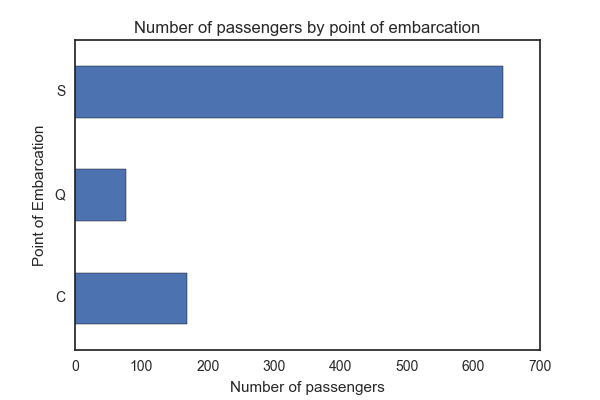
\includegraphics{NbPassengersByEmbarcationPt.png}
\caption{Diagram}
\end{figure}

\textbf{KEYS: C = Cherbourg, Q = Queenstown, S = Southampton}

    \textbf{About Duplicated data:}

The code shows that the following categorical features have duplicates:

\begin{itemize}
\item
  \textbf{Cabin}: meaning some passengers shared the same cabin.
  Moreover, some passengers have many cabins
\item
  \textbf{Ticket}: meaning some passengers were registered on the same
  ticket.
\end{itemize}

The following categorical features don't have duplicates:

\begin{itemize}
\item
  \textbf{Name}: meaning this feature could be considered as unique and
  as an identifier
\item
  \textbf{PassengerId}: this feature is redundant with the index
\end{itemize}

    \subsubsection{Relation between
features}\label{relation-between-features}

    Relation Fare vs Embarked vs Pclass
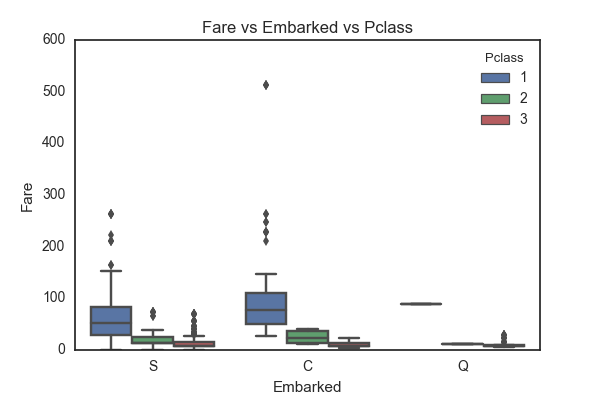
\includegraphics{boxplotFarevsEmbarkedvsPclass.png}

    Relation Survived vs Age vs Title\_Miss: It gives clues on: - Age
distribution according to Survival and - relation between Title Miss,
Survival and Age features 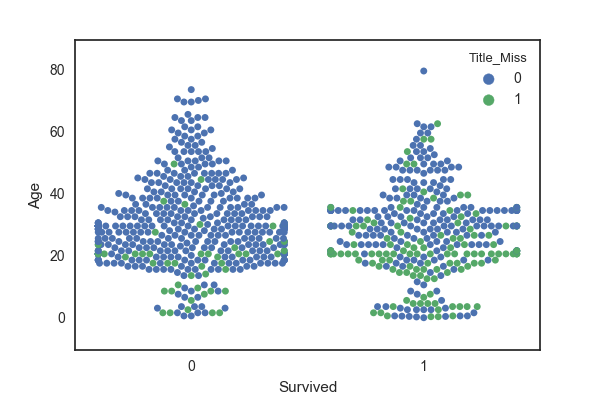
\includegraphics{SexFactorv2.png}

    Relation Survived vs Age vs Title\_Mrs: It gives clues on: - Age
distribution according to Survival and - relation between Title Mrs,
Survival and Age features

\begin{figure}
\centering
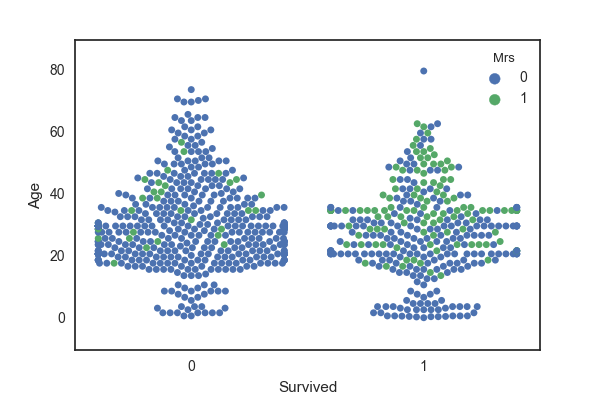
\includegraphics{SexFactorv3.png}
\caption{Diagram}
\end{figure}

    Reuse of document {[}HM{]} for building the Correlation Diagram.
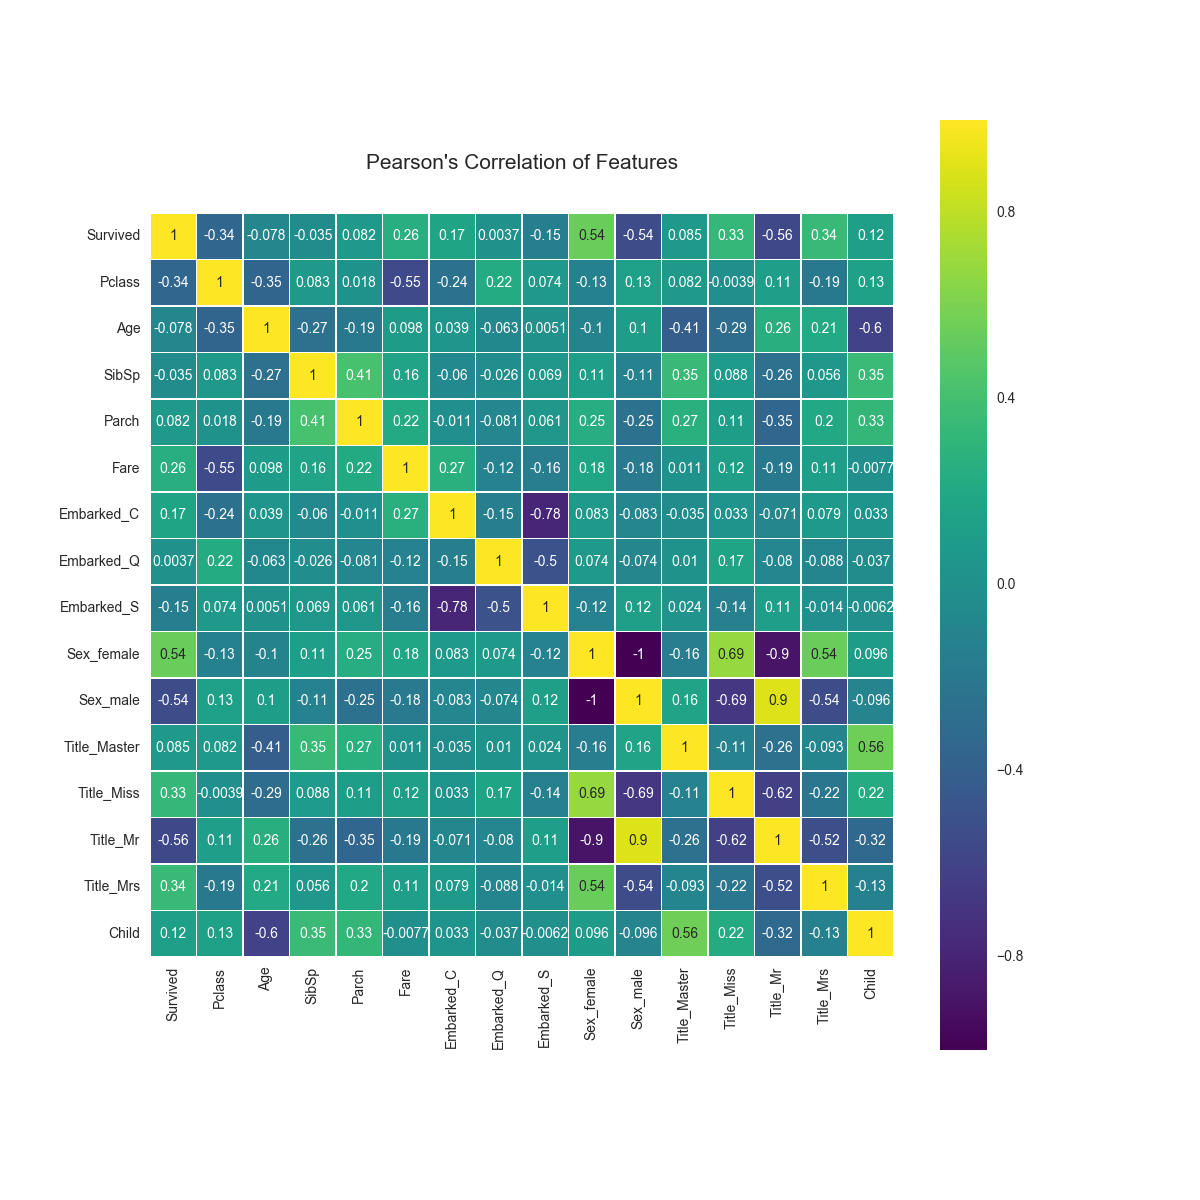
\includegraphics{PearsonCorrelationOfFeatures.png}

    \textbf{Linear Correlation deduced from Pearson's Correlation Diagram:}

Survived and Sex (female) have a linear relationship (increasing).

Survived and Title (Mr) have a linear relationship (decreasing). It is
not a surprise since Title (Mr) and Sex (female) are strongly
correlated.

Pclass and Fare have a linear relationship (decreasing).

Master and Age have a linear relationship (decreasing).

Point of Embarcation C and S have a strong linear relationship. It is
normal since Point of Embarcation C, S, Q are built from Embarked.

Age and Child have a significant linear relationship. It is normal since
child was built from Age.

SibSp and Parch have a linear relationship.

    \subsection{Importance of factors on
survival}\label{importance-of-factors-on-survival}

    \begin{figure}
\centering
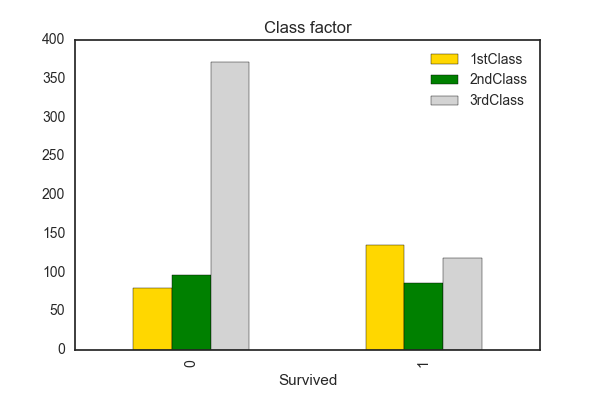
\includegraphics{ClassFactorv2.png}
\caption{Diagram}
\end{figure}

    \begin{figure}
\centering

\includegraphics{SexFactor.png}
\caption{Diagram}
\end{figure}

    \begin{figure}
\centering
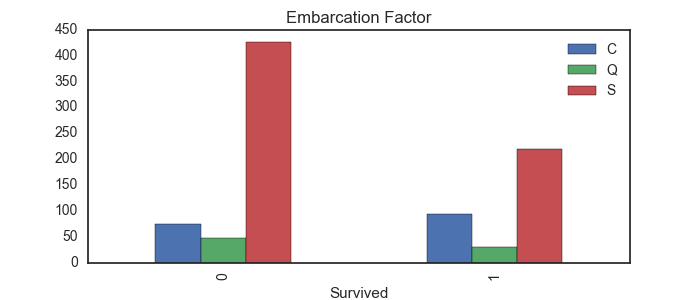
\includegraphics{EmbarcationFactor.png}
\caption{Diagram}
\end{figure}

    \begin{figure}
\centering
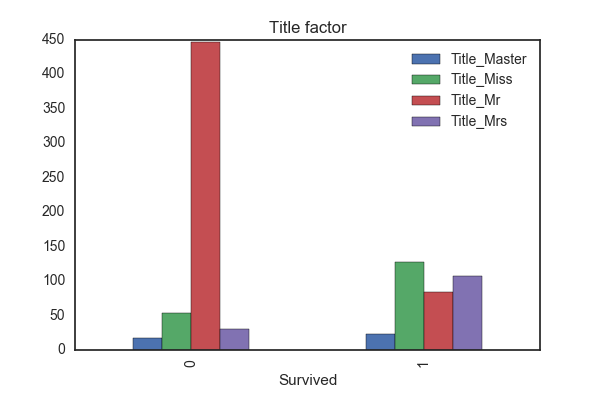
\includegraphics{TitleFactor.png}
\caption{Diagram}
\end{figure}

    \begin{figure}
\centering
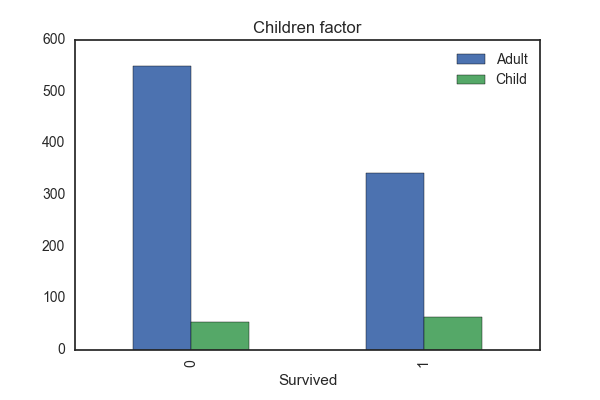
\includegraphics{ChildFactorv2.png}
\caption{Diagram}
\end{figure}

    \subsection{Answer to questions}\label{answer-to-questions}

    \begin{itemize}
\tightlist
\item
  \textbf{Q1. What are the most important factors to survival (e.g.~Sex,
  Class, \ldots{})?}
\end{itemize}

\textbf{Title}: Significantly More survival chance for Mrs, Miss and
slight more chance for Master. Significantly less survival chance for
Mr.

\textbf{Sex}: Significantly more survival chance for Sex is female.
Significantly less survival chance for sex is male.

\textbf{Class}: The first class has higher survival chance than other
classes. The third class has less chance than the two others.

\textbf{Embarked}: Point of Embarcation influences the survival chance
and Cherbourg is favored.

\textbf{Children}: Being a child (under 18) gave slightly more survival
chance.

\begin{itemize}
\tightlist
\item
  \textbf{Q2. Did they apply the protocol ``Women and Children first''?}
\end{itemize}

In document {[}Wikipedia{]} ``A disproportionate number of men were left
aboard because of a''women and children first" protocol for loading
lifeboats``. It has been applied and the figures reflect it for Women.
\textbf{The figures confirm strongly for women and slightly for
children.}

\begin{itemize}
\tightlist
\item
  \textbf{Q3. Is there any linear correlation among factors?}
\end{itemize}

To establish it is it practical to use numerical values. See here above
in Section \emph{`Relation between features'} The linear correlation
among features has been established numerically and in figure `Pearson
Correlation of Features.png' provided here above

    \begin{itemize}
\tightlist
\item
  \textbf{Q4. How to deal with missing values?}
\end{itemize}

    \begin{figure}
\centering

\includegraphics{MissingDataAmongFeatures.png}
\caption{Diagram}
\end{figure}

    High percentage of missing values for Cabin feature. \textbf{Nothing can
be done for Cabin feature.}

Significant percentage of missing values for Age feature but something
can be done for this feature. \textbf{Replace missing values for Age
with the median value of the group split by title.} See Coding in
\emph{§ Processing missing values for Age}

\begin{longtable}[]{@{}ll@{}}
\toprule
Title & Age (median)\tabularnewline
\midrule
\endhead
Master & 3.5\tabularnewline
Miss & 21.0\tabularnewline
Mr & 30.0\tabularnewline
Mrs & 35.0\tabularnewline
\bottomrule
\end{longtable}

There is a very small percentage (0.2 \%) of missing values for Embarked
feature. \textbf{For the Embarked features, replacement of the actual
values is possible (i.e.~Southampton). They have been found in document
{[}DB{]} from the name of the passengers.}

    \subsection{Way forward:}\label{way-forward}

It would be useful but not in the scope of the assignment: - MAKE
PREDICTION: to apply machine learning (e.g.~Logistic Regression) to
build a model and make prediction. - GET MORE DATA: to get more data and
split it into training and test data. The information about crew
passengers might give more insight.

    \subsection{Documentation/References}\label{documentationreferences}

Here is the list of references - including Web sites, books, blog posts
- used for my submission.

{[}Edx{]} Web site: DAT210x Programming with Python for Data Science:
\href{https://courses.edx.org/courses/course-v1:Microsoft+DAT210x+2T2017/info}{EdxSite}

{[}FE{]} Feature Engineering:
\href{https://triangleinequality.wordpress.com/2013/09/08/basic-feature-engineering-with-the-titanic-data/5}{site}

{[}DB{]} Encyclopedia Titanica database:
\href{https://www.encyclopedia-titanica.org/}{site}

{[}Wikipedia{]} Wikipedia article - See §Survivors and victims:
\href{https://en.wikipedia.org/wiki/RMS_Titanic}{wikipedia}

{[}kaggleTitanic{]} kaggle web site:
\href{https://www.kaggle.com/c/titanic/data}{kaggleTitanic}

{[}Plot{]} Matplotlib resources from Blog:
\href{http://www.datasciencecentral.com/profiles/blogs/matplotlib-cheat-sheet}{blog}

{[}Hdbk{]} Python for Data Science Handbook from Blog:
\href{http://www.datasciencecentral.com/profiles/blogs/book-python-data-science-handbook?utm_content=buffer09a5c\&utm_medium=social\&utm_source=twitter.com\&utm_campaign=buffer}{blog}

{[}HM{]} Heatmap example:
\href{https://www.kaggle.com/arthurtok/introduction-to-ensembling-stacking-in-python}{kaggle}

{[}MV{]} How to treat missing values in you data from Article:
\href{https://clevertap.com/blog/how-to-treat-missing-values-in-your-data-part-i/}{Article}


    % Add a bibliography block to the postdoc
    
    
    
    \end{document}
